\documentclass[10pt, aspectratio=169]{beamer}
\setbeamertemplate{navigation symbols}{}

\usepackage{polyglossia}

\usepackage{adjustbox}
\usepackage{amsfonts}
\usepackage{amsmath}
\usepackage{amsthm}
\usepackage{appendixnumberbeamer}
\usepackage[backend=biber,style=iso-authoryear,sortlocale=en_US,autolang=other,bibencoding=UTF8]{biblatex}
\usepackage{booktabs}
\usepackage{color}
\usepackage{csquotes}
\usepackage{datetime}
\usepackage{fontspec}
\usepackage{graphics}
\usepackage{hyperref}
\usepackage{makecell}
\usepackage{mathrsfs}
\usepackage{microtype}
\usepackage{multirow}
\usepackage{pifont}
\usepackage{fancyqr}
\usepackage[mode=buildnew]{standalone}
\usepackage{subcaption}
\usepackage{tabularx}
\usepackage{tikz}
\usepackage{todonotes}
\usepackage{ulem}
\usepackage{url}

\usetikzlibrary{arrows.meta}
\usetikzlibrary{calc}
\usetikzlibrary{shapes.geometric}

\addbibresource{zotero.bib}

\setdefaultlanguage{english}
\setotherlanguage{czech}
\setmainfont{TeX Gyre Termes}
\usetheme{Boadilla}
\usecolortheme{crane}
\setbeamertemplate{title page}[default][rounded=true,shadow=false]
\setbeamertemplate{section in toc}[ball unnumbered]
\setbeamertemplate{bibliography item}{}

\hypersetup{%
	pdfencoding=auto,
	unicode=true,
	citecolor=green,
	filecolor=blue,
	linkcolor=red,
	urlcolor=blue
}

\makeatletter
\newcommand*{\currentSection}{\@currentlabelname}
\makeatother

\def\mathdefault#1{#1}

\newcommand{\name}[1]{\textit{#1}}
\newcommand{\mathfield}{\ensuremath{\mathbb}}
\newcommand{\mathmat}{\ensuremath{\mathbf}}
\newcommand{\mathset}{\ensuremath{\mathbb}}
\newcommand{\mathspace}{\ensuremath{\mathcal}}
\newcommand{\mathvec}{\ensuremath{\bm}}

\DeclareMathOperator*{\argmin}{arg\,min}
\DeclareMathOperator*{\argmax}{arg\,max}

\newcommand{\crossmark}{\ding{56}}
\renewcommand{\checkmark}{\ding{52}}


\title[Synthetic pretraining for HPO on graphs]
{%
	Towards Synthetic Data Pretraining for Hyperparameter Optimization in Graph Learning
}

\newdate{presentation}{28}{9}{2026}
\date[September 2026]{IWCIDM@ITAT 2026, \displaydate{presentation}}

\author[Dědič \& Holeňa]
{%
	Marek~Dědič\inst{1}
	Martin~Holeňa\inst{1, 2}
}

\institute[CTU in Prague, CAS]
{%
	\inst{1} Czech Technical University in Prague \and
	\inst{2} Institute of Computer Science, Czech Academy of Sciences
}

\begin{document}

\begin{frame}
	\titlepage
\end{frame}

\begin{frame}{Parameters \& hyperparameters}
	\begin{itemize}
		\item Learners have parameters and hyperparameters
		\item Parameters optimized automatically
		\item Hyper-parameters set by humans
	\end{itemize}
	\centering
	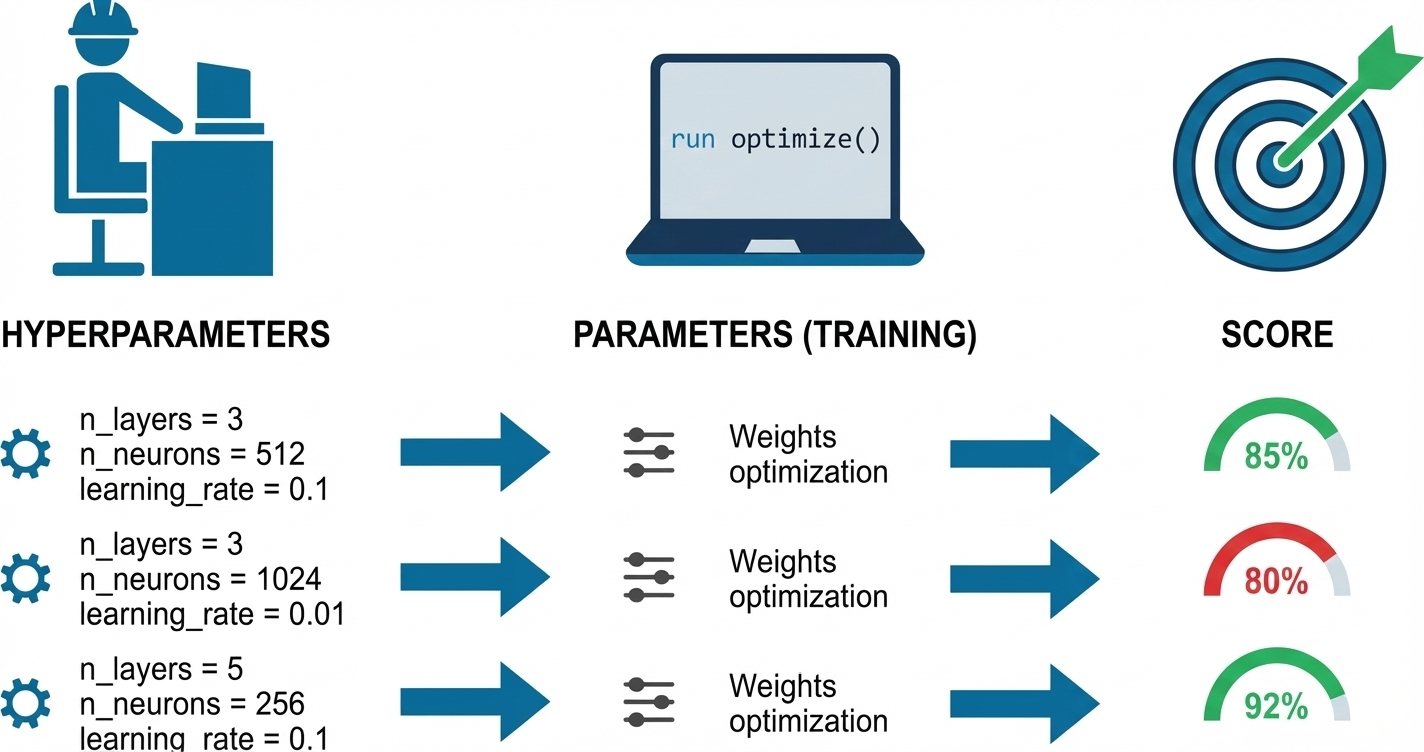
\includegraphics[width=0.5\linewidth]{images/HPO.png}\footcite{kaiku_hyperparameter_2023}
\end{frame}

\begin{frame}{GNN hyperparameter setups}
	\centering
	\only<1>{\includestandalone[width=\linewidth, page = 1]{images/hyperparameter-setups/hyperparameter-setups}}
	\only<2>{\includestandalone[width=\linewidth, page = 2]{images/hyperparameter-setups/hyperparameter-setups}}
	\only<3>{\includestandalone[width=\linewidth, page = 3]{images/hyperparameter-setups/hyperparameter-setups}}
\end{frame}

\begin{frame}{Hyper-parameter optimization}
	\begin{itemize}
		\item Hyper-parameters need to be found (semi-)automatically
		\item No gradients \( \rightarrow \) black-box problem
		\only<2>{\item \textit{Expensive} black-box problem}
		\only<3>{\item \textit{Expensive \& noisy} black-box problem}
	\end{itemize}
\end{frame}

\begin{frame}{What this talk is about}
	\textbf{Goals of this talk}:
	\begin{itemize}
		\item Show that old wisdoms about hyperparameter transfer may be wrong in some domains
		\item Explain the \textit{Cross-RF} method for hyperparameter transfer\footcite{dedic_benchmarking_2026}
		\item Explain the \textit{Synthetic-RF} method for hyperparameter transfer
		\item Experimetally check whether Synthetic-RF is viable at all
	\end{itemize}
\end{frame}

\begin{frame}{HPO loop}
	\centering
	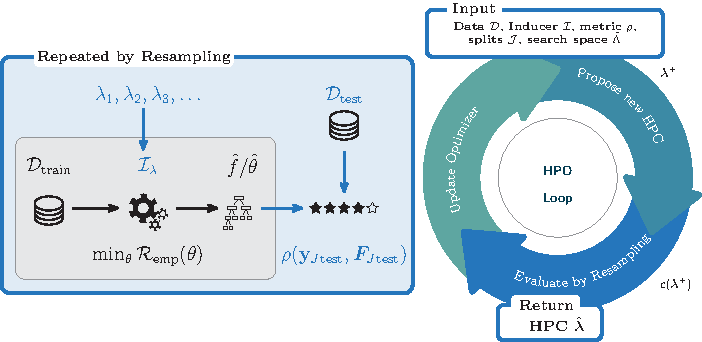
\includegraphics[width=0.8\linewidth]{images/HPO-loop.pdf}\footcite{bischl_hyperparameter_2023}
\end{frame}

\begin{frame}{HPO formalization}
	Formally, a HPO method \( \tau \) is a function that proposes a hyperparameter configuration \( \hat{\lambda} \) to try next:
	\[
		\hat{\lambda} = \tau \left( \mathcal{D}, \mathscr{F}, \tilde{\Lambda}, \rho \right)
	\]
	given
	\begin{itemize}
		\item \( \mathcal{D} \): dataset
		\item \( \mathscr{F} \): learning algorithm
		\item \( \tilde{\Lambda} \): search space
		\item \( \rho \): performance metric
	\end{itemize}
\end{frame}

\begin{frame}{The Cross-RF method\footcite{dedic_benchmarking_2026}}
	We assume that we have:
	\begin{itemize}
		\item A graph property extraction function \( \delta : \mathrm{D} \to \mathfield{R}^d \)
		\item A meta-model \( \mathcal{M}_\rho : \mathfield{R}^d \times \boldsymbol\Lambda \to \mathfield{R} \) that predicts a performance metric \( \rho \) given dataset properties and hyperparameter configuration
	\end{itemize}
	\begin{overprint}
		\onslide<2>
		We propose a HPO method using such a metamodel:
		\vspace{1em}

		\centering
		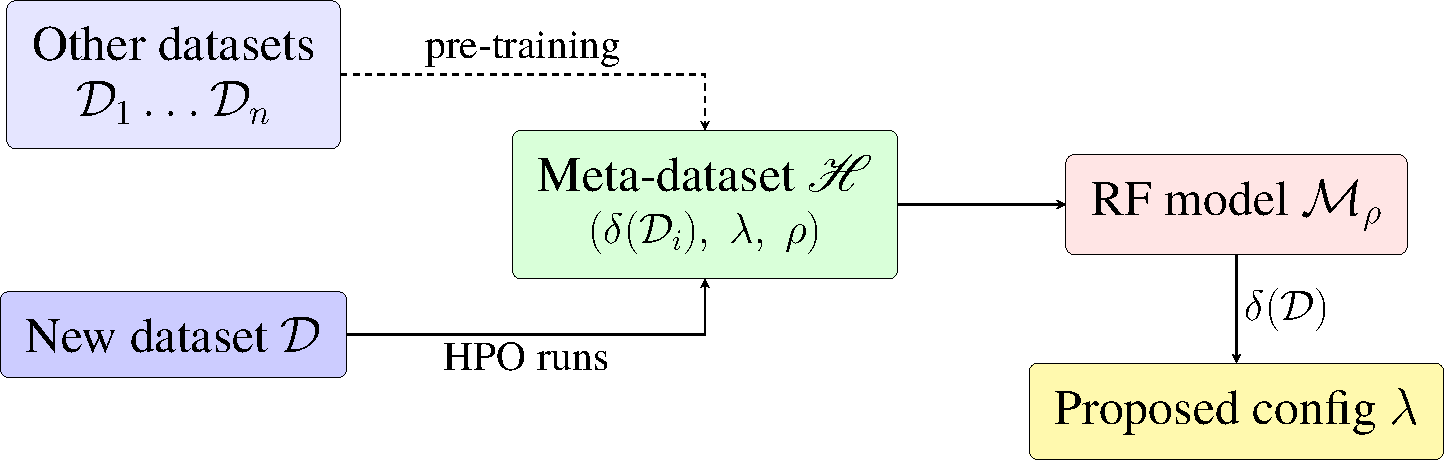
\includegraphics[width=0.8\linewidth]{images/cross-rf-overview/cross-rf-overview.pdf}

		\onslide<3>
		More formally:
		\begin{equation*}
			\tau \left( \mathcal{D}, \mathscr{F}, \tilde{\Lambda}, \rho \right) = \argmax_{\lambda \in \tilde{\Lambda}} \mathcal{M}_\rho \left( \delta \left( \mathcal{D} \right), \lambda \right)
		\end{equation*}
		Meta model is cheap \( \rightarrow \) \( \argmax \) is feasible
	\end{overprint}
\end{frame}

\begin{frame}{Meta-dataset}
	A meta-dataset used to train the metamodel:
	\begin{center}
		\resizebox{\linewidth}{!}{%
			\begin{tabular}{rrrrrrrr}
				\toprule
				\multicolumn{4}{c}{\textbf{Dataset properties}} & \multicolumn{3}{c}{\textbf{Hyper-parameters}} & \textbf{Perf.\ metrics} \\
				\cmidrule(r){1-4} \cmidrule(lr){5-7} \cmidrule(l){8-8}
				\textbf{Node count} & \textbf{Class ratio} & \textbf{\# of components} & \textbf{Avg.\ node degree} & \textbf{\# of layers} & \textbf{Dropout} & \textbf{Activation} & \textbf{F1} \\
				\midrule
				6 & 1 / 3 & 1 & 2 & 2 & 0.3 & ReLU & 0.65 \\
				6 & 1 / 3 & 1 & 2 & 3 & 0.3 & ReLU & 0.7 \\
				6 & 1 / 3 & 1 & 2 & 2 & 0.5 & ReLU & 0.62 \\
				6 & 1 / 3 & 1 & 2 & 3 & 0.5 & ReLU & 0.6 \\
				\bottomrule
			\end{tabular}
		}
	\end{center}
\end{frame}

\begin{frame}{The Cross-RF metamodel}
	Can we pretrain the metamodel on other datasets and transfer to a new one?

	\vspace{1cm}
	\hspace{1cm}\uncover<2->{\textbf{Yes.}}
\end{frame}

\begin{frame}{From Cross-RF to Synthetic-RF}
	\centering

	{\Large\textbf{Cross-RF \uncover<2->{ \( \rightarrow \) Synthetic-RF}}}

	\vspace{1em}

	\begin{tikzpicture}
		\node[anchor=south west, inner sep=0] (img) at (0,0) {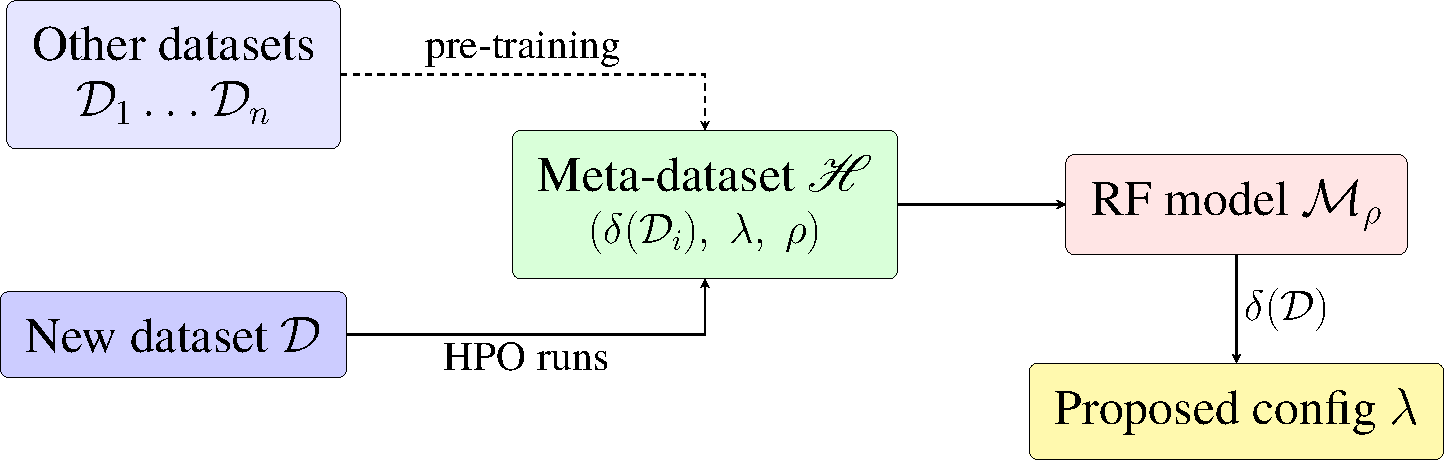
\includegraphics[width=0.8\linewidth]{images/cross-rf-overview/cross-rf-overview.pdf}};
		% Coordinates relative to the image: (0,0) = bottom left, (1,1) = top right
		\begin{scope}[x={(img.south east)}, y={(img.north west)}]
			\draw<2->[red, line width=3pt, line cap=round] (0.02,0.85) -- (0.1,0.97) (0.02,0.97) -- (0.1,0.85);
			\node<-1>[white, font=\bfseries] at (0.05,1.1) {Synthetic};
			\node<2->[font=\bfseries] at (0.05,1.1) {Synthetic};
		\end{scope}
	\end{tikzpicture}
\end{frame}

\begin{frame}{Why go synthetic?}
	\begin{itemize}
		\item Cross-RF: pretrained on a few real datasets \( \rightarrow \) target may be \textit{out-of-distribution}
		\item<2-> Synthetic-RF: \textbf{generate} the pretraining datasets \textit{around} the target
		\item<2-> Tuner unchanged, only the meta-dataset used to train \( \mathcal{M}_\rho \) changes
	\end{itemize}
	\vspace{1em}
	\centering
	\includestandalone[width=0.75\linewidth]{images/descriptor-space/descriptor-space}
\end{frame}

\begin{frame}{Generating synthetic datasets}
	Summarize the target dataset \( \mathcal{D} \) by
	\[
		\boldsymbol{s} = \left( n, \, k, \, \bar{c}, \, h, \, m \right)
	\]
	\begin{itemize}
		\item \( n \): number of nodes, \( k \): number of classes, \( \bar{c} \): average degree
		\item \( h \): edge homophily, \( m \): number of node features
	\end{itemize}
	\vspace{1em}
	\uncover<2->{%
		For each synthetic dataset, perturb the first four statistics:
		\[
			\tilde{s}_j = \mathrm{clip} \left( u_j \, s_j \right), \quad u_j \sim \mathcal{U} \left( 1 - \varepsilon, 1 + \varepsilon \right)
		\]
		Clipping keeps the target bracketed (RF cannot extrapolate)
	}
\end{frame}

\begin{frame}{Stochastic block model}
	\begin{columns}[c,onlytextwidth]
		\begin{column}{0.45\textwidth}
			\centering
			\includestandalone[width=\linewidth]{images/sbm/sbm}
		\end{column}
		\begin{column}{0.52\textwidth}
			Stochastic block model\footcite{holland_stochastic_1983} with
			\[
				p_\text{in} = \frac{\tilde{h} \, \tilde{c}}{\bar{b}}, \qquad p_\text{out} = \frac{\left( 1 - \tilde{h} \right) \tilde{c}}{\tilde{n} - \bar{b}}
			\]
			where \( \bar{b} = \tilde{n} / \tilde{k} \) is the average block size

			\vspace{1em}
			\uncover<2->{%
				Preserved in expectation:
				\begin{itemize}
					\item Average degree \( \tilde{c} \)
					\item Edge homophily \( \tilde{h} \)
				\end{itemize}
			}
		\end{column}
	\end{columns}
\end{frame}

\begin{frame}{Node features}
	\begin{itemize}
		\item Features generated conditionally on the class\footcite{guyon_design_2003}
		\item Each class \( \rightarrow \) one Gaussian cluster centred at a vertex of a hypercube
		\item All features informative, no label noise
		\item \( \tilde{m} = \max \left( m, \left\lceil \log_2 \tilde{k} \right\rceil + 1 \right) \) to fit one cluster per class
	\end{itemize}
	\vspace{1em}
	\uncover<2->{%
		Result: a complete synthetic node-classification dataset
		\begin{itemize}
			\item Train GNNs on it with various configurations \( \lambda \)
			\item Add \( \left( \delta \left( \tilde{\mathcal{D}} \right), \lambda, \rho \right) \) to the meta-dataset
			\item Pretrain the metamodel \( \mathcal{M}_\rho \) on these, then tune on \( \mathcal{D} \)
		\end{itemize}
	}
\end{frame}

\begin{frame}{Experiment setup}
	\begin{itemize}
		\item Cora dataset (2 708 nodes, 5 429 edges)
		\item GraphSAGE model with 8 hyperparameters
		\item 5 repeated iterations for each configuration
		\item HPO early-stopping based on wall-clock time \& improvement
	\end{itemize}
\end{frame}

\begin{frame}{Experiment setup}
	\begin{itemize}
		\item Used a random forrest regressor as the meta-model
		\item 100 trees, default paramers from \texttt{scikit-learn}
		\item Pretrained on 5 synthetic datasets with 30 hyperparameter configurations each
		\item In each step, all of the already evaluated configurations are excluded from \( \tilde{\Lambda} \)
		\item Compared with random search
	\end{itemize}
\end{frame}

\begin{frame}{Synthetic-RF results}
	Is the Synthetic-RF approach completely misguided?

	\vspace{1cm}
	\hspace{1cm}\uncover<2->{\textbf{No.}}

	\vspace{1cm}
	\hspace{1cm}\uncover<3->{(Random search F1-score: \( 0.8535 \), Synthetic-RF F1-score: \( 0.8628 \))}
\end{frame}

\begin{frame}{Future work}
	Immediate next steps:
	\begin{itemize}
		\item Including a broader range of GNN architectures
		\item Considering other performance metrics
		\item Comparing to newer HPO methods
		\item Consider other synthetic graph generation methods
	\end{itemize}

	Longer-term directions:
	\begin{itemize}
		\item De-couple the synthetic datasets from the target dataset
		\item Using a different metamodel architecture which is better suited to continuous search spaces
		\item Incorporating the metamodel as a surrogate model within an SMBO framework
	\end{itemize}
\end{frame}

\begin{frame}{Conclusion}
	\begin{itemize}
		\item Shown that synthetic datasets can be used to pretrain a hyperparameter optimizer for GNNs
		\item Implemented as a standard Optuna sampler
		\item More interesting research to come
	\end{itemize}
\end{frame}

\titlegraphic{%
	\begin{tikzpicture}[overlay,remember picture]
		\node[anchor=east, align=center, left=0.2cm, yshift=-1.3cm] at (current page.east){%
			\fancyqr[height=0.2\textwidth, color=black]{https://dedic.eu/publications\#dedic_towards_2026} \\
			\small More at \url{dedic.eu}
		};
	\end{tikzpicture}
}

\begin{frame}
	\titlepage
\end{frame}

\appendix

\begin{frame}[allowframebreaks]{Bibliography}
	\printbibliography
\end{frame}

\end{document}
